\subsection{Prototype 1}

\subsubsection{Presentation}
\textbf{Tools:} proto.io

\paragraph{Rationale}
This prototype focuses on a content driven display showing users immediately
what is available local to them with interactive tools for adjusting their
search.

\paragraph{Home Map}
\marginpar{%
	\null%
% \begin{figure}[htbp]
% 	\centering
	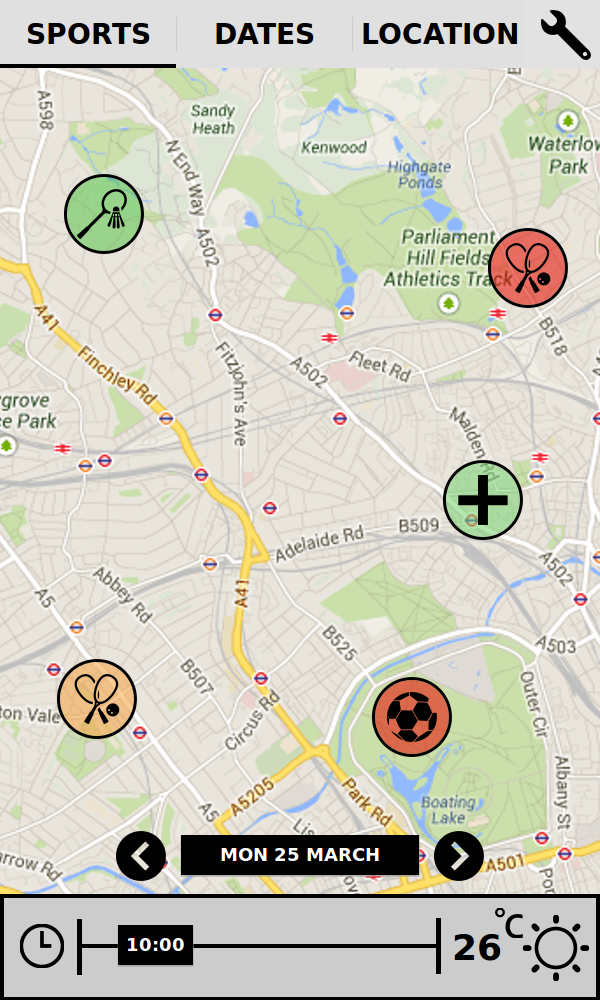
\includegraphics[width=\marginparwidth]{img/firstPrototypes/Pro1Home}
	% \caption{The home map screen}
	\captionof{figure}{The home map screen}
% \end{figure}
}
On opening the app, the user is immediately shown this map home screen with the
date and time set to the current time and the location centred on the user's
location.

\begin{enumerate}
	\item The tab bar links to pages where the user can decide which sports and
		dates to filter into the search. The location tab will prompt the user
		to enter a new postcode to centre the map on or ask them if they would
		like to reset to their current location.
	\item Icons represent locations to play sport. Where a single sport is
		available to play at a location, a picture for that sport is shown.
		Where more than one sport is available, a plus sign is show to indicate
		that several sports are available at that location. When a user presses
		a sports icon, they are shown the book now screen.
	\item Colour shows, using a traffic light scale, either:
		\begin{enumerate}
			\item availability of courts/facilities. Green indicates there is
				full availability at the location where red indicates there is
				only one booking left at this time.
			\item price of bookings at this location. Green indicates all
				bookings are free at this location and red indicates prices are
				expensive (in comparison to other activities in the area).
		\end{enumerate}

	\item Settings button brings up a small drop down box to ask the user which
		of the two options they would like colour to indicate, availability or
		price.
	\item Map is navigable in the same way as the phone's native map
		application.  The user can zoom in and out with finger gestures and pan
		left, right, up and down. As the user changes their location/zoom
		level, the sports icons update to cover the new area.
	\item The current day being shown, with arrows to navigate through all days
		which are selected in the dates tab. By default, this is all dates, but
		the user can filter the dates via the dates tab.
	\item A time slider which can be moved in hour increments. The icons shown
		on the map will change to accurately show what bookings are available
		for the hour following whatever time this slider is set to by the user.
	\item A weather prediction for the date and time currently selected.
\end{enumerate}

\paragraph{Sports filter}
\marginpar{%
	\null%
% \begin{figure}[htbp]
% 	\centering
	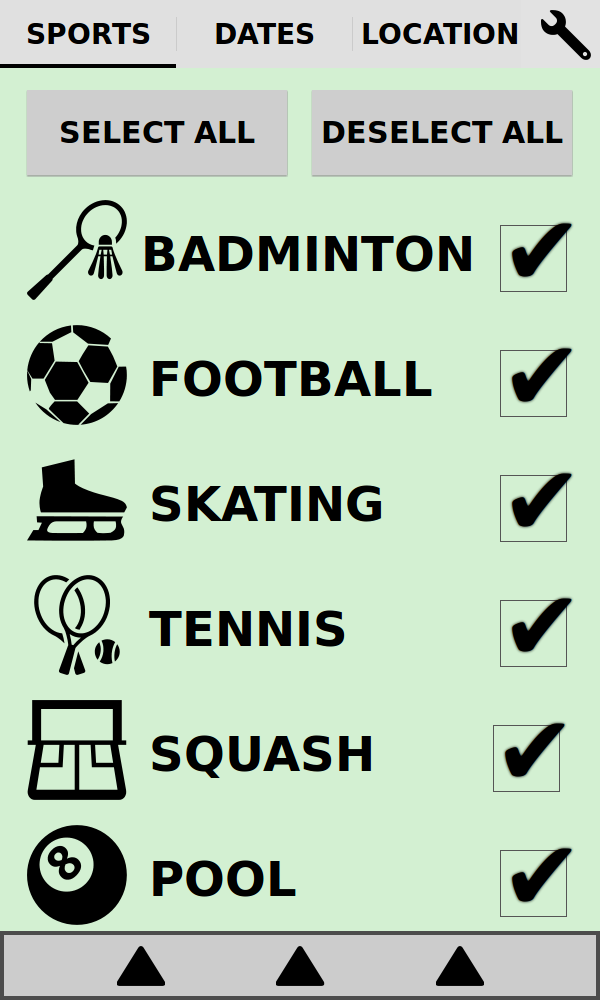
\includegraphics[width=\marginparwidth]{img/firstPrototypes/Pro1Sports}
	\captionof{figure}{Sports filter screen}
% \end{figure}
}

A page to filter which sports are shown on the map home page.

\begin{enumerate}
	\item Buttons for quickly selecting or deselecting all sports.
	\item Checkboxes; when ticked, the chosen sports are included in the
		search.
	\item A bar that can be either pressed or dragged up to close the sports
		selection tab and return to the map home page.
	\item The tab bar remains so the user can navigate between sports, date and
		location selection without having to do so via the home screen.
\end{enumerate}

\paragraph{Dates filter}
\marginpar{%
	\null%
% \begin{figure}[htbp]
% 	\centering
	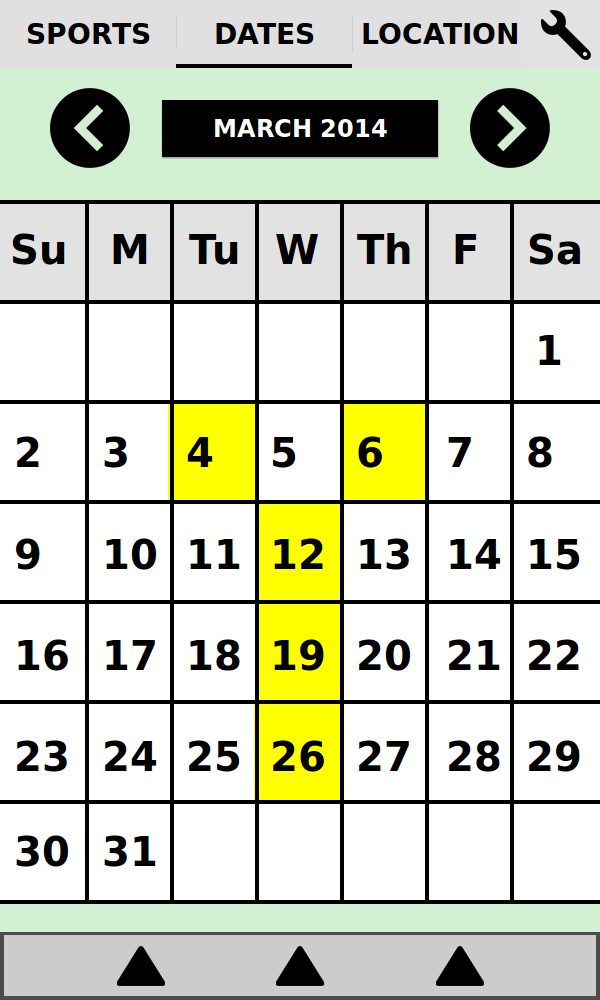
\includegraphics[width=\marginparwidth]{img/firstPrototypes/Pro1Dates}
	\captionof{figure}{Dates filter screen}
% \end{figure}
}

A page to filter which dates are included in the search. Dates which are
highlighted are included in the date navigation on the map home page. (no 4 on
the home screen)

\begin{enumerate}
	\item Arrows to move between months of the year.
	\item Days of the month. A user can press a number to highlight it, or
		swipe around the screen to highlight several dates in one swipe, e.g.\
		swiping across a whole row to highlight an entire week.
	\item Days of the week. A user can press one of these days, such as M for
		monday, to highlight every occurrence of that day in the month.
	\item A bar that can be either pressed or dragged up to close the dates
		selection tab and return to the map home page.
	\item The tab bar remains so the user can navigate between sports, date and
		location selection without having to do so via the home screen.
\end{enumerate}

\paragraph{Book now screen}

This screen appears when a user selects a sports icon on the home page. The
screen does not cover the whole of the previous page, allowing the user to
still see the date of the booking and the weather prediction for that time. The
user can press the x to close this screen and return to the search.

\marginpar{%
	\null%
% \begin{figure}[htbp]
% 	\centering
	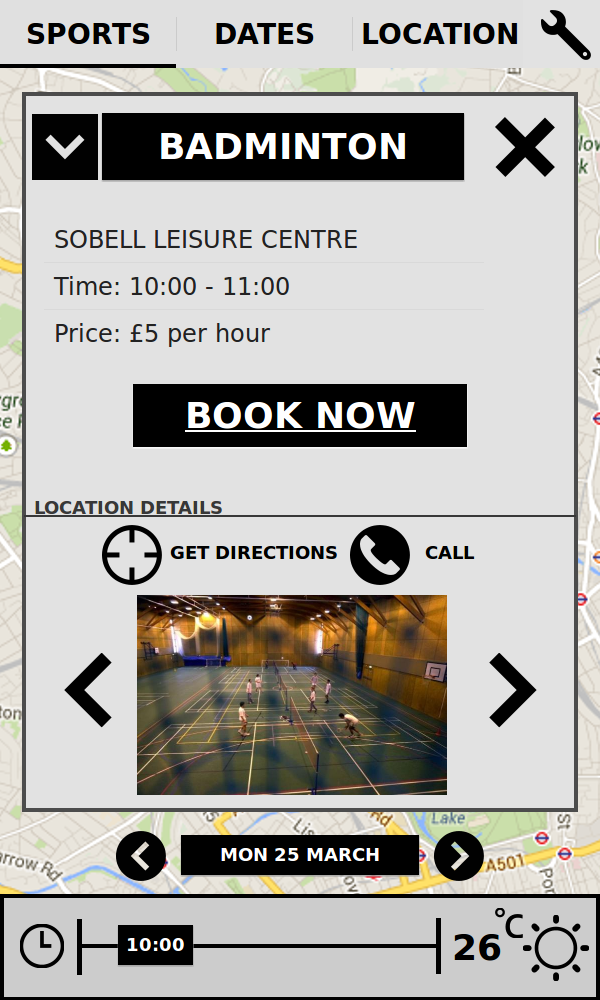
\includegraphics[width=\marginparwidth]{img/firstPrototypes/Pro1Booking}
	\captionof{figure}{Book now screen}
% \end{figure}
}
% \begin{figure}[htbp]
% 	\centering
% 	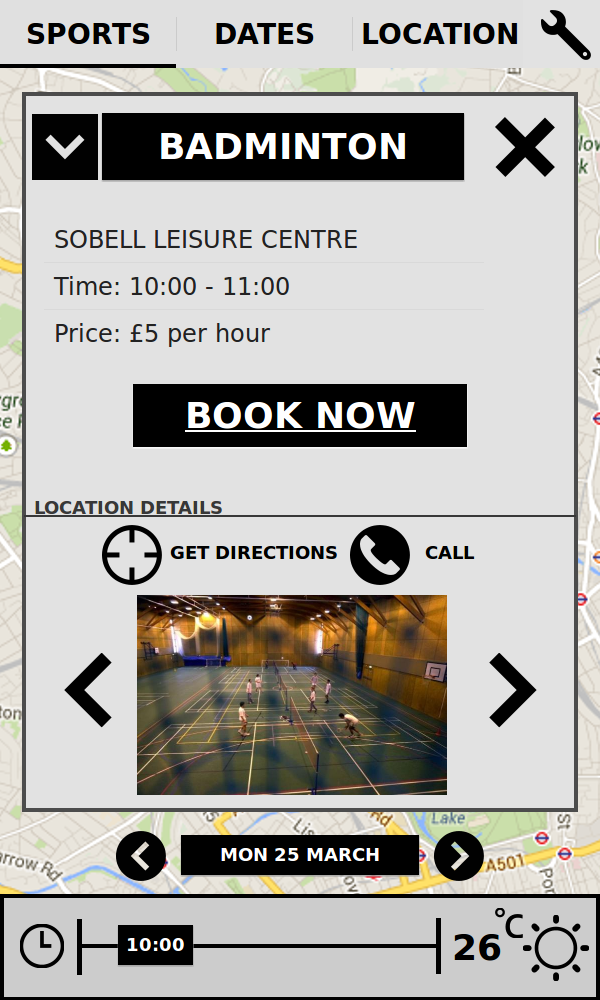
\includegraphics[width=0.25\paperwidth]{img/firstPrototypes/Pro1Booking}
% 	\caption{Book now screen}
% \end{figure}

\begin{enumerate}
	\item The sport available at this location. If several sports are available
		at this location, a drop down arrow is show next to the sport name to
		allow the user to select other sports at that location.
	\item User can get directions through their phone's native map application,
		call the reception of the offices to get more information or navigate
		through pictures of the facilities.
	\item The user can still attempt to change the time or date on the screen.
		If a booking slot is available at the newly selected time then details
		on the book now screen will change to reflect the change in time and
		price (if applicable). If a booking is not available then the text
		between the sport name and `Location Details' will be replaced by a
		message telling the user no booking is available at this time.
	\item The `Book Now' can be pressed to take the user to an external pay
		site or the website of that sports facility to pay for the booking.
\end{enumerate}

\newgeometry{left=3cm}
\subsubsection{Evaluation}

\begin{center}
	\renewcommand{\arraystretch}{2}
	\begin{longtable}{p{0.3\textwidth} c p{0.6\textwidth}}
		\toprule
		\textbf{Criteria} & \textbf{Rating} & \textbf{Comment}\\
		\midrule
		Visibility of system status & $+$ & The time and date of the current
		results are always shown on the home screen.\\

		Match between system and the real world & + & Map applications have
		become ubiquitous so use of the map should be intuitive.\\

		User control and freedom & 0 & There are intuitive ways to return to
		previous screens and navigate between screens. However, an undo or
		return button could be added to return a user to a previous page they
		were on.\\

		Consistency and standards & $-$ & May not be clear that the dates on
		the map screen correspond to those in the dates filter tab.\\

		Error prevention & 0 & Relatively few screens reduces the number of
		places an error can be made. Ensure there is a confirmation message
		before letting the user book facilities.\\

		Recognition rather than recall & 0 & Clear icons are used to indicate
		each sport. No indication on map screen of which dates they can scroll
		through unless they go to the dates tab to see selected dates.\\

		Flexibility and efficiency of use & 0 & Swiping on dates filter tab can
		speed up date selection. No bulk booking, if user knows they want to
		make several bookings, they have to search and process each
		indiviually. \\

		Aesthetic and minimalist design & + & Keeping sports and date filters
		tabs separate from map results and grouping icons when several sports
		are available leaves map search results clear from clutter.\\

		Help users recognize, diagnose, and recover from errors & $-$ & If a
		user changes time or date on the booking screen they will be shown a
		message if a booking is not available at that time. However, there is
		no undo button to return to the original selection.\\

		Help and documentation & $-$ & Currently no descriptions or tutorials
		telling the user how to use they system. Could add a help icon which
		allows users to see what each page does or an initial tutorial on first
		use of the application.\\
		\bottomrule
	\end{longtable}
\end{center}

\begin{center}
	\renewcommand{\arraystretch}{2}
	\begin{longtable}{p{0.12\textwidth} p{0.3\textwidth} c p{0.45\textwidth}}
		\toprule
		\textbf{User} & \textbf{Scenario} & \textbf{Rating} & \textbf{Comment}\\
		\midrule
		\textbf{Elderly} & Searching for new sports in the area & 0 & Howard is
		given an immediate visual representation of what sports are available
		near him when opening the app. However, with his lack of experience
		with technology, use of the map may not be intuitive to him and he may
		prefer options to read results as a list.\\

		& Raquet sport with 4 friends on friday & 0 & Howard could tick only
		racquet sports on the sports filter tab and fridays on the dates tab.
		However, there is no way for him to bulk book if he wants to regularly
		play.\\

		& Swimming nearby with knee pain & $-$ & There is currently no way to
		search for facilities that have disabled access. This could be included
		in the description of the facility on the booking page but Howard would
		still have to look at each search result individually.\\

		\midrule
		\textbf{Working} & Team sport on friday & + & Janet can select the
		relevant sports and dates to show relevant results.  Could have quick
		buttons on the sports tab screen to quick select all team sports to
		speed this up.\\

		& Change/cancel booking at late notice & $-$ & As booking payments are
		held outside the application there is currently no way to cancel
		bookings or even see previous bookings. Could add a screen to add
		favourite booking slots to so users can potentially see previous
		bookings.\\

		& Outdoor sport early saturday & + & Janet can select the relevant
		sports and dates to show relevant results.Could have quick buttons on
		the sports tab screen to quick select all outdoor sports to speed this
		up. The weather prediction on the map screen also helps inform her
		search here.\\

		\midrule
		\textbf{Student} & Tennis court at specific times & + & Jenny can
		select tennis from the sports tab and all preferred dates from the
		dates tab and then quickly browse through her options on the map. \\

		% across different times at the weekend.\\
		& Weekday evening session & + & Jenny can select all days from the date
		tab then set the time to evening on the map and scroll through each day
		seeing which day suits her best.\\

		\midrule
		\textbf{Child} & Outdoor sport close to home or on a bus route & 0 & If
		Joe chooses his preferred outdoor sports from the sports tab, he will
		be shown those close to him straight away. However, there is no
		indication of bus routes on the map. An option could be added to
		overlay local bus routes on the map.\\

		& Booking several squash courts for after school tournament & $-$ &
		There is no way for Joe to book several courts at one time or several
		dates at one time. Could add an option on the booking screen to book
		several courts at once or add a basket function so users can select all
		the bookings they want and then pay for them together.\\

		& Could have some kind of rating system to the location description on
		the bookings page and some way to search for highly rated locations.\\
		\bottomrule
	\end{longtable}
\end{center}
\restoregeometry

\subsubsection{Conclusion}

%\noindent Description of features to take forward + changes that can
%be made to these features and features to avoid because of their failings
%etc.
